% \documentclass[aspectratio=169, 11pt]{beamer}
\documentclass[aspectratio=169, 11pt, handout]{beamer}

% ── Theme ──
\usetheme{Madrid}
\usecolortheme{default}
\setbeamertemplate{navigation symbols}{}
\setbeamertemplate{footline}{%
  \leavevmode\hbox{%
    \begin{beamercolorbox}[wd=.333333\paperwidth,ht=2.5ex,dp=1ex,center]{author in head/foot}%
      \usebeamerfont{author in head/foot}\insertshortauthor
    \end{beamercolorbox}%
    \begin{beamercolorbox}[wd=.333333\paperwidth,ht=2.5ex,dp=1ex,center]{title in head/foot}%
      \usebeamerfont{title in head/foot}\insertshorttitle
    \end{beamercolorbox}%
    \begin{beamercolorbox}[wd=.333333\paperwidth,ht=2.5ex,dp=1ex,right]{date in head/foot}%
      \usebeamerfont{date in head/foot}\insertframenumber{} / \inserttotalframenumber\hspace*{2ex}
    \end{beamercolorbox}}}

% ── Packages ──
\usepackage{amsmath,amssymb}
\usepackage{booktabs}
\usepackage{xcolor}
\usepackage{colortbl}
\usepackage{graphicx}
\usepackage{tikz}
\usetikzlibrary{arrows.meta, positioning, calc}

% ── Colors ──
\definecolor{sbgreen}{HTML}{00704A}  % course accent
\definecolor{warnred}{HTML}{CC0000}
\definecolor{noteblue}{HTML}{2060A0}

% ── Commands ──
\newcommand{\E}{\mathbb{E}}
\newcommand{\Var}{\mathrm{Var}}
\newcommand{\Cov}{\mathrm{Cov}}
\newcommand{\SE}{\mathrm{SE}}
\newcommand{\Prob}{\mathrm{Pr}}
\newcommand{\indep}{\perp\!\!\!\perp}

\usepackage{soul}
\newcommand{\NUM}[2]{\sethlcolor{yellow}\hl{#1\,\textsuperscript{?}}\marginpar{\tiny #2}}
% Beamer frames are typeset inside boxes, where \marginpar raises "Not in outer par mode"
% and \marginparwidth is 4pt. Same marker; the provenance note goes to the frame footnote.
\renewcommand{\NUM}[2]{\sethlcolor{yellow}\hl{#1\,\textsuperscript{?}}\footnote[frame]{\tiny #2}}
% Compact footnote layout so several provenance notes fit under one frame.
\setbeamertemplate{footnote}{\noindent\raggedright\hspace*{0.6em}\tiny\insertfootnotemark\,\insertfootnotetext\par}

% Version 2 (2026-09-29). Course spine: estimand -> identification -> estimation.
% Case C re-skin: the floor-lead staffing model is now an AI assistant for store associates.
% Changes from slides.tex: m10/CHANGES-v2.md.
\newcommand{\spinestep}[1]{\textcolor{sbgreen}{\textbf{#1}}}

% ── Title ──
\title[Meeting 10]{Meeting 10: Before, After, and Everyone Else}
\subtitle{Applied Causal Inference for Business}
\author{Zhikun Lu}
\date{\today}

\begin{document}

% ====================================================================
\begin{frame}
\titlepage
\end{frame}

% ====================================================================
\begin{frame}{Where Does the Counterfactual Come From?}

\begin{center}
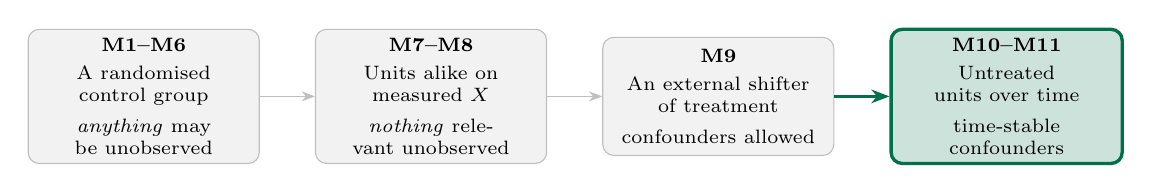
\begin{tikzpicture}[
    node distance=0.45cm and 0.7cm,
    box/.style={draw, rounded corners, minimum width=2.9cm, minimum height=1.5cm,
                font=\scriptsize, align=center, text width=2.7cm},
    active/.style={box, fill=sbgreen!20, draw=sbgreen, very thick},
    inactive/.style={box, fill=gray!10, draw=gray!50}
]
\node[inactive] (A) {\textbf{M1--M6}\\[2pt] A randomised control group\\[3pt] \emph{anything} may be unobserved};
\node[inactive, right=of A] (B) {\textbf{M7--M8}\\[2pt] Units alike on measured $X$\\[3pt] \emph{nothing} relevant unobserved};
\node[inactive, right=of B] (C) {\textbf{M9}\\[2pt] An external shifter of treatment\\[3pt] confounders allowed};
\node[active, right=of C] (D) {\textbf{M10--M11}\\[2pt] Untreated units over time\\[3pt] time-stable confounders};

\draw[-{Stealth}, gray!50] (A) -- (B);
\draw[-{Stealth}, gray!50] (B) -- (C);
\draw[-{Stealth}, thick, sbgreen] (C) -- (D);
\end{tikzpicture}
\end{center}

\bigskip

\begin{center}
\small M9 needed an instrument someone designed. Today nobody designed anything.\\
The comparison is the same stores \emph{before}, and other stores over the \emph{same weeks}.
\end{center}
\end{frame}

% ====================================================================
\begin{frame}{Today's Plan}

\begin{center}
\small
\begin{tabular}{rll}
\toprule
\textbf{Minutes} & \textbf{Block} & \\
\midrule
0--60 & A & \textbf{Exam II} (M6--M9) \\
70--120 & B & Difference-in-differences: the $2 \times 2$, its assumption, its interval; then TWFE \\
130--180 & C & \textbf{Lab 4:} an agent loop for experiment review \\
\bottomrule
\end{tabular}
\end{center}

\bigskip

\textbf{Block B, on the spine:}
\begin{enumerate}\small
    \item \spinestep{Estimand:} the AI assistant's effect on cohort 1, written with go-live dates --- and the number that settles cohort 2
    \item \spinestep{Identification:} parallel trends, no anticipation, no spillovers --- \emph{assumptions}, not design
    \item \spinestep{Estimation:} the pre-period check, store- and region-level SEs, the drift that would change the decision; the within transformation and TWFE; auditing a report
\end{enumerate}

\bigskip

\textbf{Case:} Dana's AI assistant rollout, part 1 (Releases 1--5). \quad \textbf{At home:} the panel core, with Notebook 10 (72 hours). \quad \textbf{Released:} P4; Lab 5 (self-paced).
\end{frame}

% ====================================================================
\begin{frame}{Exam II: M6--M9}

\begin{center}
\begin{tabular}{rl}
\toprule
0--3 & Instructions and questions about the paper \\
3--58 & \textbf{55 minutes} of work \\
58--60 & Papers collected; break until 70 \\
\bottomrule
\end{tabular}
\end{center}

\bigskip

\textbf{Examinable:} the slides of M6--M9 and Section~1 of each set of notes. Section~3 of the notes, anything marked \emph{Extension}, and regression discontinuity are not.

\bigskip

\textbf{The one habit that earns marks:} in every question, find the \emph{number that decides it} before computing anything, and say which comparison produced it --- and for whom.
\end{frame}

% ====================================================================
\section{The Estimand: The Rollout}
% ====================================================================

% [RELEASE R1 — narrative, cost parameters, the analyst's two numbers; flagship held out]
% [RELEASE R1 — narrative, cost parameters, the analyst's two numbers and the vendor's dashboard; flagship held out]
\begin{frame}{The Store Assistant}

\textbf{Dana} runs store operations for a home-goods chain of 120 stores. \textbf{Store Assistant} is a generative-AI assistant on associates' handhelds: stock checks, product answers, add-on suggestions, in seconds.

\medskip

In week 53 the first \textbf{cohort of thirty stores} went live. A second cohort of thirty is scheduled for \textbf{week 79}. It is now week 78. {\small (The flagship went live much earlier, alone. It is held out today; M11 gives it its own hour.)}

\pause
\medskip

\textbf{On her desk:} confirm cohort 2 --- \textyen 2{,}500 per store-week (licence \textyen 1{,}700, handsets \textyen 300, the store's ``AI champion'' \textyen 500), thirty stores, from next week.

\begin{center}
\small
\begin{tabular}{lr}
\toprule
Analyst: cohort 1, weekly sales after going live against before & $+$\textyen 15{,}000 \\
Analyst: cohort 1 against the other stores, after going live & $+$\textyen 41{,}000 \\
Vendor dashboard: ``AI-assisted sales'' in cohort 1 stores & \textyen 38{,}000 \\
\bottomrule
\end{tabular}
\end{center}

\small Analyst: \emph{``Either way, it pays several times over.''} \quad Vendor: \emph{``Assisted sales are fifteen times the fee.''}
\end{frame}

% ====================================================================
\begin{frame}{The Number That Decides It}

The assistant costs \textyen 2{,}500 per store-week. Gross margin on incremental sales is \textbf{25\%}.

\bigskip

The model pays in a store-week only if it adds sales worth more than its cost:
\[
0.25 \times \Delta\text{sales} \;>\; 2{,}500 .
\]

\bigskip
\pause

\begin{alertblock}{Break-even lift}
\[
\Delta^{*} \;=\; \frac{2{,}500}{0.25} \;=\; \textbf{\textyen 10{,}000 per store-week}
\]
\end{alertblock}

\bigskip

Both of the analyst's numbers clear it easily. Every estimate today is a weekly sales lift. The only question is \textbf{which side of \textyen 10{,}000} it lands on.

\small \textbf{The dashboard is not a third estimate.} It counts sales in which the assistant was \emph{used} --- including the customer who came in for the frying pan anyway. Usage is not impact: M1's Sure Thing, in a vendor's report. And even at face value, \textyen 38{,}000 of sales is \textyen 9{,}500 of margin: 3.8 times the fee, not fifteen.
\end{frame}

% ====================================================================
% [RELEASE R2 — four-cell table; worksheet attempt before the next frame]
\begin{frame}{Four Numbers}

Mean weekly sales per store, \textyen 000. The comparison stores are the 89 not yet on the model.

\bigskip

\begin{center}
\begin{tabular}{lrr}
\toprule
& \textbf{Before} (weeks 27--52) & \textbf{After} (weeks 53--78) \\
\midrule
Cohort 1 (30 stores) & 181 & 196 \\
Comparison (89 stores) & 151 & 155 \\
\bottomrule
\end{tabular}
\end{center}

\bigskip

\textbf{In pairs}, compute and commit in writing:

\begin{enumerate}
    \item cohort 1, after minus before
    \item after adoption, cohort 1 minus the comparison stores
    \item the change in cohort 1 minus the change in the comparison stores
\end{enumerate}

\bigskip

Which of the three does Dana put against \textyen 10{,}000?
\end{frame}

% ====================================================================
\begin{frame}{Before, Across, and Both}

\begin{center}
\begin{tabular}{llr}
\toprule
\textbf{Comparison} & \textbf{Arithmetic} & \textbf{\textyen 000} \\
\midrule
Before/after & $196 - 181$ & \textcolor{warnred}{15} \\
Across stores & $196 - 155$ & \textcolor{warnred}{41} \\
\textbf{Difference-in-differences} & $(196 - 181) - (155 - 151)$ & \textcolor{sbgreen}{\textbf{11}} \\
\bottomrule
\end{tabular}
\end{center}

\pause
\medskip

Each wrong number is the right one plus something else:
\begin{align*}
15 &= 11 + \underbrace{4}_{\text{what every store did anyway}} \\
41 &= 11 + \underbrace{30}_{\text{cohort 1 stores were bigger before}}
\end{align*}

\pause

Before/after keeps the \textbf{trend}. Across keeps the \textbf{level}. The DiD removes the level by differencing each group over time, and the trend by differencing the groups.

\medskip

\begin{center}
Against \textyen 10{,}000: \textbf{11}. Not ``several times over'' --- by \textyen 1{,}000.
\end{center}
\end{frame}

% ====================================================================
\begin{frame}{Three Steps for a Rollout}

Index potential outcomes by the week a store goes live: $Y_{it}(g)$, with $g = \infty$ for a store that never does.

\begin{center}
\small
\begin{tabular}{p{2.8cm}p{9.8cm}}
\toprule
\spinestep{Estimand} & $\text{ATT} = \E\bigl[Y_{it}(53) - Y_{it}(\infty) \mid G = 53\bigr]$, weeks 53--78: what the assistant did for cohort 1, against \textyen 10{,}000. \\[0.5em]
\spinestep{Identification} & \textbf{No coin chose the go-live dates.} Identification comes from an \emph{assumption} about untreated trends: parallel trends, no anticipation, no spillovers. It can be checked in part, never proved. \\[0.5em]
\spinestep{Estimation} & The $2 \times 2$ difference; TWFE for the full panel; SEs at the level the rollout was assigned --- the store, or the region. \\
\bottomrule
\end{tabular}
\end{center}

\bigskip

M1--M6 had the design do step 2. M7--M9 argued it from a recorded rule or a coin. Today it rests on a claim about what \emph{would have} happened to trends.
\end{frame}

% ====================================================================
\begin{frame}{Borrowing the Comparison's Trend}

Quarterly means, \textyen 000. Cohort 1 adopts at the start of Q5.

\begin{center}
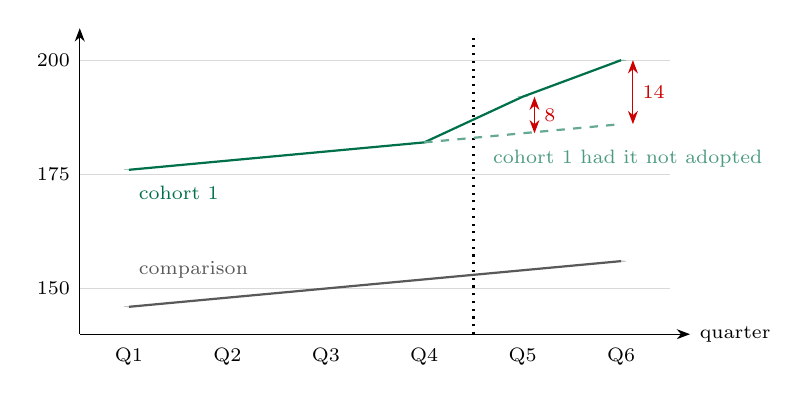
\begin{tikzpicture}[xscale=1.25, yscale=0.058]
\draw[-{Stealth}] (0.5,140) -- (6.7,140) node[right, font=\scriptsize] {quarter};
\draw[-{Stealth}] (0.5,140) -- (0.5,207);
\foreach \x in {1,...,6} {\node[font=\scriptsize] at (\x,135) {Q\x};}
\foreach \y in {150,175,200} {\node[font=\scriptsize, anchor=east] at (0.5,\y) {\y}; \draw[gray!30] (0.5,\y) -- (6.5,\y);}
\draw[dotted, thick] (4.5,140) -- (4.5,205);
\draw[thick, gray!70!black] (1,146) -- (2,148) -- (3,150) -- (4,152) -- (5,154) -- (6,156);
\foreach \x/\y in {1/146,2/148,3/150,4/152,5/154,6/156} {\fill[gray!70!black] (\x,\y) circle (1.5pt);}
\draw[thick, sbgreen] (1,176) -- (2,178) -- (3,180) -- (4,182) -- (5,192) -- (6,200);
\foreach \x/\y in {1/176,2/178,3/180,4/182,5/192,6/200} {\fill[sbgreen] (\x,\y) circle (1.5pt);}
\draw[thick, dashed, sbgreen!60] (4,182) -- (5,184) -- (6,186);
\draw[{Stealth}-{Stealth}, warnred] (5.12,184) -- (5.12,192) node[midway, right, font=\scriptsize] {8};
\draw[{Stealth}-{Stealth}, warnred] (6.12,186) -- (6.12,200) node[midway, right, font=\scriptsize] {14};
\node[font=\scriptsize, sbgreen, anchor=west] at (1,171) {cohort 1};
\node[font=\scriptsize, gray!70!black, anchor=west] at (1,154) {comparison};
\node[font=\scriptsize, sbgreen!70, anchor=west] at (4.6,178.5) {cohort 1 had it not adopted};
\end{tikzpicture}
\end{center}

\pause

The dashed line is the comparison's path, \textbf{shifted up by the gap of 30}. That is the whole identifying move: cohort 1's own level, the comparison's trend.
\end{frame}

% ====================================================================
\begin{frame}{What Must Be True}

\begin{alertblock}{Identifying assumption: parallel trends}
Had cohort 1 not adopted, its sales would have changed by the same amount as the comparison stores':
\[
\E\bigl[Y_{\text{after}}(0) - Y_{\text{before}}(0) \mid \text{cohort 1}\bigr] \;=\; \E\bigl[Y_{\text{after}}(0) - Y_{\text{before}}(0) \mid \text{comparison}\bigr] .
\]
\end{alertblock}

\bigskip
\pause

\textbf{Levels may differ. Trends may not.} Anything that shifts a store's level for good --- size, location, format --- cancels. Anything that moves a group's \emph{trend} does not.

\bigskip

Two more, less dramatic but not optional:
\begin{itemize}
    \item \textbf{No anticipation.} Cohort 1's ``before'' is not already affected by the assistant --- or by preparing for it.
    \item \textbf{No spillovers.} The assistant in one store does not move a comparison store's sales.
\end{itemize}
\end{frame}

% ====================================================================
\begin{frame}[shrink=3]{The Assumptions, Sentence by Sentence}

From Dana's rollout file:

\bigskip

\begin{center}
\small
\begin{tabular}{p{6.8cm}p{6.2cm}}
\toprule
\textbf{The case says} & \textbf{Which buys --- or risks} \\
\midrule
``Cohorts were assigned by region, in the order the regional managers signed off, after each region's data-privacy review.'' & Timing not chosen by a store --- but parallel trends becomes a claim about \emph{regions}. \\[0.4em]
``Associates were trained on the assistant in weeks 51--52, in paid sessions off the shop floor.'' & No anticipation, \emph{if} training did not thin the floor. \\[0.4em]
``The comparison stores are the 89 whose regions had not yet signed off.'' & Same format and calendar; their levels do not matter. \\[0.4em]
``Licences are tied to store handsets; no two stores share a catchment.'' & No spillovers. \\[0.4em]
``Once the assistant took over stock checks, store managers re-planned their rotas.'' & A warning: staff hours are now \emph{caused} by the assistant. \\
\bottomrule
\end{tabular}
\end{center}

\bigskip
\pause

\textbf{Hold onto the first sentence.} Why did cohort 1's region sign off first?
\end{frame}

% ====================================================================
\begin{frame}{Three Ways Parallel Trends Fails}

\begin{center}
\small
\begin{tabular}{p{3.3cm}p{5.2cm}p{4.2cm}}
\toprule
\textbf{Failure} & \textbf{At the chain} & \textbf{Effect on the DiD} \\
\midrule
Different growth & cohort 1's region was growing faster anyway & credits the model with the region's growth \\[0.4em]
A dip, then recovery & the region signed off \emph{because} of a bad quarter & credits the model with the rebound \\[0.4em]
Composition & stores open or close in one group mid-panel & compares different stores before and after \\
\bottomrule
\end{tabular}
\end{center}

\bigskip
\pause

None of these is about levels. Each is a reason the \textbf{order of sign-off} might be related to where sales were heading.

\bigskip

The first two leave traces \emph{before} adoption. The third is visible in the store counts. None is ruled out by the $2 \times 2$ itself.
\end{frame}

% ====================================================================
\section{Estimation: Checking and Pricing}
% ====================================================================

% [RELEASE R3 — six quarters; worksheet attempt on the event-time row]
\begin{frame}{Checking the Pre-Period}

\begin{center}
\small
\begin{tabular}{lrrrr|rr}
\toprule
& \textbf{Q1} & \textbf{Q2} & \textbf{Q3} & \textbf{Q4} & \textbf{Q5} & \textbf{Q6} \\
\midrule
Cohort 1   & 176 & 178 & 180 & 182 & 192 & 200 \\
Comparison & 146 & 148 & 150 & 152 & 154 & 156 \\
\midrule
Gap & 30 & 30 & 30 & 30 & 38 & 44 \\
Gap minus Q4's gap & 0 & 0 & 0 & \textit{base} & \textcolor{sbgreen}{8} & \textcolor{sbgreen}{14} \\
\bottomrule
\end{tabular}
\end{center}

\pause
\medskip

\begin{itemize}
    \item \textbf{Before adoption the gap does not move.} No differential growth, no dip. The pre-period is where the first two failures would show.
    \item \textbf{After adoption it opens by 8, then 14.} The model ramps: below break-even in its first quarter, above in its second.
    \item The four-cell DiD of 11 is the average of the two: a fact about the window, not the model.
\end{itemize}
\end{frame}

% ====================================================================
\begin{frame}{Store-Level Standard Errors}

The panel is 119 stores $\times$ 78 weeks $=$ 9{,}282 store-weeks. A store's sales this week predict its sales next week.

\bigskip

Treating store-weeks as independent counts the same store 78 times: the standard error comes out \textbf{far too small}.

\pause
\bigskip

\textbf{The fix, by hand.} Collapse each store to one number, its change $\Delta_i = \bar Y_{i,\text{after}} - \bar Y_{i,\text{before}}$:
\[
\widehat{\text{DiD}} = \bar\Delta_{\text{cohort 1}} - \bar\Delta_{\text{comparison}} = 15 - 4 = 11 .
\]
Now it is a two-sample comparison of 30 and 89 stores. With store-level standard deviations of 6 and 5:
\[
\SE = \sqrt{\tfrac{6^2}{30} + \tfrac{5^2}{89}} = \sqrt{1.20 + 0.28} = 1.22, \qquad 11 \pm 2.4 = [8.6,\; 13.4] .
\]

\pause

\textbf{It straddles 10.} The unit of independence is the store, not the store-week. (If whole regions share shocks, not even the store is enough: next slide.)
\end{frame}

% ====================================================================
\begin{frame}{When Regions Share Shocks}

The first case sentence again: cohorts were assigned \textbf{by region}. Cohort 1 is 3 regions; the comparison stores are in 9.

\bigskip

A regional promotion, a local closure, a heatwave: shocks that hit every store in a region together. Then stores in a region are not independent either, and the store-level SE is \textbf{too small}.

\pause
\bigskip

\textbf{The same fix, one level up.} Collapse to one change per region: 3 against 9. With region-level standard deviations of 3 and 2.5:
\[
\SE = \sqrt{\tfrac{3^2}{3} + \tfrac{2.5^2}{9}} = \sqrt{3.00 + 0.69} = 1.92, \qquad 11 \pm 2.23 \times 1.92 = [6.7,\; 15.3] ,
\]
using the $t$ distribution with $3 + 9 - 2 = 10$ degrees of freedom.

\pause
\medskip

\begin{center}
\textbf{Cluster at the level the treatment was assigned.} With twelve clusters the answer is honest and wide; the notes give the wild cluster bootstrap for this case.
\end{center}
\end{frame}

% ====================================================================
\begin{frame}{Flat Is Not Proof: Trend Sensitivity}

Suppose cohort 1's region drifts up by $\delta$ per quarter relative to the comparison, too slowly to see before adoption. The DiD compares Q5--Q6 with Q3--Q4, two quarters apart, so it absorbs $2\delta$:

\begin{center}
\small
\begin{tabular}{lrrrr}
\toprule
$\delta$ (\textyen 000 per quarter) & 0 & 0.25 & 0.5 & 1.0 \\
\midrule
DiD net of the drift, $11 - 2\delta$ & 11.0 & 10.5 & \textbf{10.0} & 9.0 \\
\bottomrule
\end{tabular}
\end{center}

\pause
\medskip

\begin{alertblock}{The breakdown drift}
$\delta^* = (11 - 10)/2 = 0.5$: \textyen 500 per store-week per quarter --- \textbf{\textyen 2{,}000 per store-week over a year}.
\end{alertblock}

\pause
\medskip

Would the pre-period have shown it? A drift of 0.5 moves the gap by 1.5 from Q1 to Q4, about one store-level standard error. \textbf{Flat pre-trends cannot rule it out.}

\smallskip

The report states $\delta^*$ and argues from the case whether a regional drift that large is plausible. It prices the doubt; it does not remove it.
\end{frame}

% ====================================================================
\begin{frame}{Parallel in Yuan, or in Percent?}

Parallel trends is a claim in \textbf{some units}. The comparison grew by 4 on 151, which is $2.6\%$.

\bigskip

\begin{center}
\small
\begin{tabular}{llr}
\toprule
\textbf{Counterfactual for cohort 1} & \textbf{Arithmetic} & \textbf{Effect} \\
\midrule
Same change in yuan & $181 + 4 = 185$ & $196 - 185 = 11.0$ \\
Same change in percent & $181 \times 155/151 = 185.8$ & $196 - 185.8 = 10.2$ \\
\bottomrule
\end{tabular}
\end{center}

\pause
\bigskip

When levels differ, the two cannot both hold. The choice moved the effect by \textyen 800, most of the margin over break-even.

\bigskip

Pick the scale in which the trends were parallel \emph{before} --- here yuan: the Q1--Q4 gaps are flat in yuan, and in percent they shrink from $20.5\%$ to $19.7\%$ --- and say so.
\end{frame}

% ====================================================================
\section{Estimation: Within and TWFE}
% ====================================================================

\begin{frame}{The Within Transformation}

Your warm-up, as a model. Every store has its own level; every week has its own chain-wide shock:
\[
Y_{it} = \alpha_i + \lambda_t + \beta D_{it} + \varepsilon_{it}, \qquad D_{it} = \mathbf{1}\{\text{store } i \text{ live on the assistant in week } t\}.
\]

\pause

\begin{itemize}
    \item Subtract each store's own mean: $\alpha_i$ disappears --- the \textbf{level} of 30.
    \item Subtract each week's mean across stores: $\lambda_t$ disappears --- the \textbf{trend} of 4.
    \item What is left of $D_{it}$ is variation within store \emph{and} within week. $\widehat\beta$ is the slope of what is left of $Y$ on it --- FWL again (M8).
\end{itemize}

\pause
\bigskip

This is \textbf{two-way fixed effects} (TWFE). The fixed effects are the DiD's two subtractions, written as a regression so that it runs on 9{,}282 rows with controls and standard errors attached.

\small With store effects alone, the coefficient is cohort 1's own change, $15$: only cohort 1's cells vary in $D$. Week effects bring in the comparison's $+4$, giving $11$. One-pass demeaning is exact only in a \textbf{balanced} panel; with closures, run the regression with both sets of effects.
\end{frame}

% ====================================================================
\begin{frame}{With One Adoption Date, TWFE Is the $2 \times 2$}

Double-demean the four cells: subtract row mean and column mean, add back the grand mean.

\begin{center}
\small
\begin{tabular}{lrr|rr}
\toprule
& \multicolumn{2}{c|}{$\ddot Y$} & \multicolumn{2}{c}{$\ddot D$} \\
& Before & After & Before & After \\
\midrule
Cohort 1 & $-2.75$ & $2.75$ & $-0.25$ & $0.25$ \\
Comparison & $2.75$ & $-2.75$ & $0.25$ & $-0.25$ \\
\bottomrule
\end{tabular}
\end{center}

\vspace{-0.3em}
\[
\widehat\beta_{\text{TWFE}} = \frac{\sum \ddot D\,\ddot Y}{\sum \ddot D^{\,2}} = \frac{4 \times 0.25 \times 2.75}{4 \times 0.0625} = \textbf{11} = (196 - 181) - (155 - 151) .
\]

\pause

\begin{alertblock}{With a single adoption date}
TWFE \textbf{is} the four-cell difference-in-differences. Four cells, four parameters: the regression reproduces the table exactly. On all six quarters it is the post-period gap minus the pre-period gap, $41 - 30 = 11$.
\end{alertblock}

\small M11: when stores adopt on different dates, this equality breaks --- and not harmlessly.
\end{frame}

% ====================================================================
\begin{frame}{The Event-Study Regression}

Replace the single $D_{it}$ by one indicator per quarter for cohort 1, leaving Q4 out as the base:
\[
Y_{it} = \alpha_i + \lambda_t + \sum_{k \neq 4} \beta_k\, \mathbf{1}\{i \in \text{cohort 1}\}\,\mathbf{1}\{t \in \text{Q}k\} + \varepsilon_{it} .
\]

\pause

\begin{center}
\small
\begin{tabular}{lrrrrrr}
\toprule
& $\beta_1$ & $\beta_2$ & $\beta_3$ & \textit{base} & $\beta_5$ & $\beta_6$ \\
\midrule
Six-quarter table & 0 & 0 & 0 & --- & 8 & 14 \\
\bottomrule
\end{tabular}
\end{center}

\bigskip

\begin{itemize}
    \item With one adoption date, each $\beta_k$ \textbf{is} the quarter-$k$ gap minus the Q4 gap: the last row of the six-quarter table.
    \item The pre-period coefficients are the parallel-trends check; the post-period ones are the ramp.
    \item One regression, both jobs --- and the base period is a choice to report.
\end{itemize}
\end{frame}

% ====================================================================
% [RELEASE R4 — the store-week panel; collect predictions before the ladder]
\begin{frame}{The Store-Week Panel}

\begin{center}
\small
\begin{tabular}{lrl}
\toprule
& \textbf{Stores} & \textbf{On the model} \\
\midrule
Cohort 1 & 30 & from week 53 \\
Cohort 2 & 30 & not before week 79: comparison today \\
Never scheduled & 59 & comparison \\
Flagship & 1 & held out \\
\midrule
Store-weeks, weeks 1--78 & \multicolumn{2}{l}{$119 \times 78 = 9{,}282$} \\
\bottomrule
\end{tabular}
\end{center}

\bigskip

\textbf{Predict before you look.} In pairs, write down:

\begin{enumerate}
    \item TWFE with store and week effects, weeks 1--78, \textyen 000
    \item its standard error treating store-weeks as independent, and clustered by store
    \item the event-study coefficients for Q5 and Q6
\end{enumerate}

\begin{center}\small Commit before the next slide.\end{center}
\end{frame}

% ====================================================================
\begin{frame}{The Ladder}

\begin{center}
\small
\begin{tabular}{lr}
\toprule
\textbf{Estimate, weeks 1--78} & \textbf{\textyen 000 / store-week} \\
\midrule
Cohort 1, after minus before & \textcolor{warnred}{\NUM{16.1}{sim staffing-panel v1: cohort-1 mean, weeks 53--78 minus 27--52}} \\
Cohort 1 minus comparison, after & \textcolor{warnred}{\NUM{42.3}{sim staffing-panel v1: post-period cross-section difference}} \\
TWFE, store $+$ week effects & \NUM{12.4}{sim staffing-panel v1: TWFE on cohort 1 and 89 comparison stores, weeks 1--78} \\
\quad SE, store-weeks independent \;/\; clustered by store & \NUM{0.3}{sim staffing-panel v1: iid OLS SE} \;/\; \NUM{1.2}{sim staffing-panel v1: store-clustered SE} \\
Event study: largest $|\beta_k|$ before adoption; $\beta_5$; $\beta_6$ & \NUM{0.5}{sim staffing-panel v1: max abs pre-period quarter coefficient} ;\; \NUM{11.2}{sim staffing-panel v1: Q5 coefficient} ;\; \NUM{13.8}{sim staffing-panel v1: Q6 coefficient} \\
\bottomrule
\end{tabular}
\end{center}

\pause

\begin{itemize}\small
    \item Store and week effects took out the level and the trend, as on the four cells.
    \item Clustering by store multiplied the SE by four. The interval now reaches down to break-even.
    \item Pre-period coefficients are flat; the ramp is there, faster than the hand table's.
\end{itemize}
\end{frame}

% ====================================================================
\section{The Report}
% ====================================================================

% [RELEASE R5 — the analyst's draft; audit attempt before the answers]
% [RELEASE R5 — the analyst's draft; audit attempt before the answers]
\begin{frame}{The Analyst's Draft}

Seven sentences from the draft memo. \textbf{In pairs:} for each, say what is wrong, or that nothing is.

\bigskip

\begin{enumerate}\small
    \item ``Cohort 1 sales rose by \textyen 16{,}100 per store-week after going live.''
    \item ``On 9{,}282 store-weeks the effect is significant at $p < 0.001$ (SE 0.3).''
    \item ``We control for weekly staff hours, which differ across stores.''
    \item ``Stores that closed during the period were dropped.''
    \item ``The pre-period is weeks 1--52.''
    \item ``Pre-period coefficients are flat, so parallel trends holds.''
    \item ``The vendor's dashboard confirms the result: assisted sales of \textyen 38{,}000 per store-week.''
\end{enumerate}

\bigskip

\begin{center}\small Commit before the next slide.\end{center}
\end{frame}

% ====================================================================
\begin{frame}{The Audit, Answered}

\begin{center}
\scriptsize
\begin{tabular}{p{4.0cm}p{8.9cm}}
\toprule
\textbf{Sentence} & \textbf{Problem, and the fix} \\
\midrule
1. Rose by 16.1 & Before/after: keeps the chain's own trend. Report the DiD. \\[0.3em]
2. $p < 0.001$ on 9{,}282 rows & Store-weeks are not independent. Cluster by store: SE 1.2, and the interval reaches 10. \\[0.3em]
3. Controls for staff hours & Managers re-planned rotas \emph{because of} the assistant: a post-treatment control (M7). It absorbs part of the effect. \\[0.3em]
4. Closed stores dropped & Fine only if closures are unrelated to the rollout. Report closures by group; a balanced panel changes who is compared. \\[0.3em]
5. Pre-period weeks 1--52 & Training ran in weeks 51--52, off the floor. If it thinned service, those weeks are not ``before''. End the base period at week 50 and check. \\[0.3em]
6. Flat, so it holds & Flat pre-trends are consistent with parallel trends, not proof. Report $\delta^*$. \\[0.3em]
7. The dashboard confirms & Usage, not impact: no comparison group, counts sales that would have happened anyway, and it is the vendor's number. It confirms nothing. \\
\bottomrule
\end{tabular}
\end{center}

\pause
\medskip

\small Four are about \textbf{what was compared}; one about \textbf{the interval}; one about \textbf{what was assumed}; one about \textbf{whose number it is}. None is about the estimator.
\end{frame}

% ====================================================================
\section{The Decision}
% ====================================================================

\begin{frame}{Dana's Table}

In \textyen 000 per store-week; break-even $10$.

\begin{center}
\scriptsize
\begin{tabular}{llrl}
\toprule
\textbf{Estimate} & \textbf{What it contains} & \textbf{Lift} & \textbf{Reading} \\
\midrule
After minus before & effect $+$ chain trend & \NUM{16.1}{sim v1: cohort-1 before/after} & \textcolor{warnred}{not causal} \\
Cohort 1 minus comparison & effect $+$ level gap & \NUM{42.3}{sim v1: post cross-section} & \textcolor{warnred}{not causal} \\
TWFE, store-clustered & average, 26 post-weeks & \NUM{12.4 (1.2)}{sim v1: TWFE; store-clustered SE} & \textcolor{sbgreen}{above}; interval touches 10 \\
Event study, Q5 / Q6 & first / second quarter & \NUM{11.2}{sim v1: Q5} / \NUM{13.8}{sim v1: Q6} & ramp; Q6 clearly above \\
Trend sensitivity & drift that erases the margin & \NUM{0.8}{(TWFE $-$ 10)/3: sim TWFE; pre and post midpoints three quarters apart} per quarter & state and argue \\
\bottomrule
\end{tabular}
\end{center}

\pause
\medskip

\small The hand table and the panel agree on the \textbf{sign}, the \textbf{ramp} and a \textbf{thin} average margin. The average hides that the second quarter is where the money is.
\vspace{1.0em}
\end{frame}

% ====================================================================
\begin{frame}{The Recommendation}

\begin{block}{To Dana}
Confirm cohort 2 for week 79 and keep the regions on their schedule. The event study puts the lift at \NUM{11.2}{sim v1: Q5} then \NUM{13.8}{sim v1: Q6} thousand per store-week against a break-even of 10 --- in margin, about $+$\textyen 300 then $+$\textyen 950 per store-week.
\end{block}

\pause

\textbf{Four sentences the memo must contain.}
\begin{enumerate}\small
    \item The estimate assumes cohort 1's region would have tracked the comparison stores. Pre-period coefficients are flat; a regional drift of \textyen \NUM{800}{sim v1: trend-sensitivity breakdown, yuan per store-week per quarter} per store-week per quarter would erase the average margin.
    \item Clustered by region, the interval is wider still and includes 10.
    \item Cohort 2's regions signed off \emph{later}. If sign-off tracked expected sales, cohort 1 overstates what cohort 2 will see.
    \item The vendor's ``assisted sales'' measure use, not effect, and are not part of the evidence.
\end{enumerate}

\end{frame}

% ====================================================================
\begin{frame}{Key Takeaways}

\begin{itemize}
    \item \spinestep{Estimand.} Write it with go-live dates: $\E[Y_{it}(53) - Y_{it}(\infty) \mid G = 53]$. A vendor's usage metric is not an estimate of it.
    \item \spinestep{Identification.} No design chose the dates: parallel trends, no anticipation and no spillovers are \emph{assumptions}. Tie them to why the treated were chosen \emph{when} they were. The pre-period checks; it does not prove --- report $\delta^*$.
    \item \spinestep{Estimation.} Before/after keeps the trend; across keeps the level; the DiD removes both (15 and 41 against 11). With one adoption date, TWFE is the $2 \times 2$. The unit of independence is the store, or the region.
    \item \textbf{Put the interval in margin.} \textyen 12{,}400 of sales, SE 1{,}200, is $-$\textyen 350 to $+$\textyen 850 a store-week.
\end{itemize}
\end{frame}

% ====================================================================
\begin{frame}{Take-Home Panel Core}

Done at home (30--45 minutes), submitted with Notebook 10 within 72 hours. Everything you need is on these slides; nothing is left to the lab.

\bigskip

\begin{enumerate}\small
    \item From the six-quarter table, compute each quarter's gap minus the Q4 gap, and the post-period average DiD. Say what the average hides.
    \item Double-demean the four cells by hand and confirm $\widehat\beta_{\text{TWFE}} = 11$.
    \item With store-level standard deviations of 6 and 5, compute the 95\% interval for the DiD. Does it clear 10?
    \item Trend sensitivity: find $\delta^*$ for the post-average DiD, and for the Q6 gap alone (base Q3--Q4). Which conclusion is more robust, and why?
    \item Rewrite the analyst's memo in five sentences: the number, its interval, the assumption, $\delta^*$, and the decision.
\end{enumerate}

\bigskip

\textbf{Submit} with Notebook 10. \quad \textbf{IV or panel project pairs:} revised identification plan due 72 hours after today.
\end{frame}

% ====================================================================
\begin{frame}{Lab 4: An Agent That Reviews an Experiment}

The simulated experimentation platform from Lab 3. Fifty minutes.

\medskip

\begin{center}
\scriptsize
\begin{tabular}{rlp{8.6cm}}
\toprule
\textbf{Min} & \textbf{Slot} & \textbf{Task} \\
\midrule
5  & Task and specification & The agent's job: read an experiment's design document and draft readout, query the records, and return a verdict with its evidence. Write the verdict schema. \\
10 & Demonstration & A loop: plan, call a tool, record what was found, decide whether to continue. \\
25 & Build & Your loop, with the Lab 3 tools, on three experiments: one clean, one with a sample-ratio mismatch, one with a switched primary metric. \\
7  & Verify & Against the known answers: did it flag the two problems, and leave the clean one alone? \\
3  & Interpret & One sentence: which check the agent skipped, and how the evidence log showed it. \\
\bottomrule
\end{tabular}
\end{center}

\small \textbf{Close:} an agent's verdict is only as good as the checks it runs --- steps 1--3, automated. This is P4, released tonight. \textbf{Lab 5} (self-paced, evaluation-driven development) is released too. Model, access and platform details: the lab handout and syllabus appendix.
\end{frame}

\end{document}
